\section{AC-DC Converter Design and Analysis}

\subsection{}
$
    f = \qty{50}{\hertz} \\
    V_{mains} = \qty{230}{\volt_{RMS}} \\
    V_{out} = \qty{30}{\volt} \\
    V_{ripple} = \qty{6}{\volt} \\
    I_{out} = \qty{5}{\ampere}
$

Firstly, the peak voltage needs to be found to determine what ratio is required for the step-down transformer.
\begin{align*}
    \hat{V} & = \sqrt{2} V_{RMS}                \\
            & = \sqrt{2} \cdot \qty{230}{\volt} \\
            & = \qty{325.269}{\volt}
\end{align*}
To find the transformer specifications, the peak voltage can be divided by the desired output plus half
the permitted ripple. This returns the ratio of windings.
\begin{align*}
    N_{ratio} & = \frac{\hat{V}}{V_{out} + \frac{1}{2}V_{ripple}}             \\
              & = \frac{\qty{325.3}{\volt}}{\qty{30}{\volt} + \qty{3}{\volt}} \\
              & = 9.86
\end{align*}
Rounded down to allow some buffer for voltage drops across components during rectification and filtering,
it is found that a ratio of 9.5:1 (19:2) provides a voltage of \qty{34.24}{\volt}. Each diode must be rated above
this to prevent reverse breakdown. Furthermore, the load circuit requires \qty{5}{\ampere} of current. The diodes
must be rated at ten times this ($\sim\qty{50}{\ampere}$) due to peak pulsed current draw by the capacitor.

Full-bridge rectification means that two diodes are conducting each half cycle. Each drops \qty{0.7}{\volt}.
The peak voltage after rectification is \qty{32.84}{\volt}, meaning the voltage across the load
should be \qty{29.84 \pm 3}{\volt} given correct capacitor choice.

Using only capacitor smoothing, the minimum value can be found:
\begin{align*}
    C & = \frac{\hat{I}}{2 f \cdot \Delta V}                                        \\
      & = \frac{ \qty{5}{\ampere} }{ 2 \cdot \qty{50}{\hertz} \cdot \qty{6}{\volt}} \\
      & = \qty[parse-numbers=false]{8.\overline{3}}{\milli\farad}
\end{align*}

% \hfill \break
This results in the following circuit: \vspace{5mm}

\begin{center}
    \begin{circuitikz}[
            american,
            % circuitikz/voltage/american,
            circuitikz/straight=true,
            full diodes,
            circuitikz/diodes/scale=0.5
        ]
        \ctikzset{quadpoles/transformer/height=2.15}
        \ctikzset{transformer L1/.style={inductors/coils=7, inductors/width=1.4}}
        \ctikzset{transformer L2/.style={inductors/coils=5, inductors/width=1}}
        % v source
        \draw (0,0) to [sV,v<=$\qty{230}{\volt_{RMS}}$] ++(0,3) -- ++(1,0)
        node[transformer, anchor=A1](T){19:2};
        \draw (T.A2) to [short] (0,0);
        % transformer output
        \draw (T.B1) -- ++(2,0) -- ++(0,-0.5) coordinate(bridge top);
        % diode bridge
        \draw (bridge top) to [D, *-*, v^=$\qty{0.7}{\volt}$] ++(1,-1) coordinate(bridge right)
        to [D, *-*, invert] ++(-1,-1) coordinate(bridge bottom)
        to [D, *-*, invert] ++(-1,1) coordinate(bridge left)
        to [D, *-*] (bridge top);
        % bridge to trans
        \draw (bridge bottom) -- ++(0,-0.5) to [short] (T.B2);
        % capacitor
        \draw (bridge right) to [short] ++(2,0) coordinate(cap top)
        to [C, l=$\qty{8.4}{\milli\farad}$, *-*] ++(0,-2) coordinate(cap bottom)
        to [short] ++(-4,0) -- (bridge left);
        % load
        \draw (cap top) to [short] ++(1.5,0)
        to [short, i=$\qty{5}{\ampere}$] ++(1,0)
        to [open, o-o, v=$\sim\qty{30}{\volt}$] ++(0,-2)
        -- (cap bottom);
        % voltage drops        
        \draw (T.B1) to [open, v=$\qty{34.2}{\volt}$] (T.B2);
        \draw (bridge right) ++(0.5,0) to [open, v=$\qty{32.8}{\volt}$] ++(0,-2);
    \end{circuitikz}
\end{center}

The voltage and current at the source are demonstrated by the following two graphs:

\begin{center}
    \fbox{
        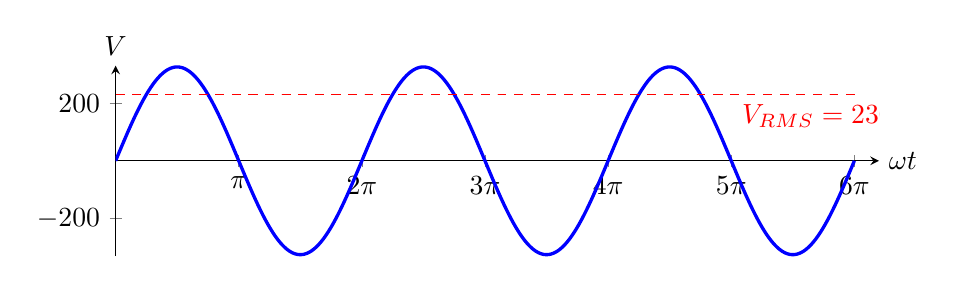
\begin{tikzpicture}
            \begin{axis}[
                    domain=0:6*pi,
                    samples=3*360,
                    xtick={0, pi, 2*pi, 3*pi, 4*pi, 5*pi, 6*pi},
                    xticklabels={\(0\), \(\pi\), \(2\pi\), \(3\pi\), \(4\pi\), \(5\pi\), \(6\pi\)},
                    width=0.93\textwidth, height=4cm,
                    ymin=-330,
                    ymax = 330,
                    xmax = 6.2*pi,
                    axis lines = center,
                    xlabel style={right},
                    ylabel style={above},
                    ylabel={$V$},
                    xlabel={$\omega t$}
                ]
                \addplot [very thick, blue] {325.269*sin(deg(x))};
                \addplot [dashed, mark=none, red]{230} node[below, pos=0.95]{$V_{RMS} = \qty{230}{\volt}$};
            \end{axis}
        \end{tikzpicture}
    }

    Source voltage

    \fbox{
        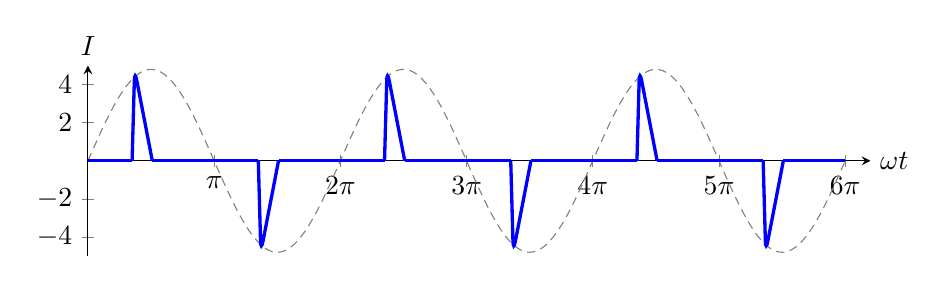
\begin{tikzpicture}
            \begin{axis}[
                    domain=0:6*pi,
                    xtick={0, pi, 2*pi, 3*pi, 4*pi, 5*pi, 6*pi},
                    xticklabels={\(0\), \(\pi\), \(2\pi\), \(3\pi\), \(4\pi\), \(5\pi\), \(6\pi\)},
                    width=0.95\textwidth, height=4cm,
                    ymin=-5,
                    ymax = 5,
                    xmax = 6.2*pi,
                    axis lines = center,
                    xlabel style={right},
                    ylabel style={above},
                    ylabel={$I$},
                    xlabel={$\omega t$}
                ]
                \addplot [densely dashed, gray, samples=3*360] {4.8*sin(deg(x))};

                \foreach \n in {0,2*pi,4*pi}
                    {
                        \addplot [very thick, blue,domain=\n:\n + 0.35*pi] {0};
                        \addplot [very thick, blue,rounded corners,samples=100] coordinates{
                                (\n +0.35*pi,0)
                                (\n +0.37*pi,4.8)
                                (\n +0.51*pi,0)
                            };
                        % \addplot [very thick, blue] coordinates{
                        %     (\n+0.51*pi,0.55)
                        %     (\n+0.51*pi,0)
                        % };
                        % \addplot [very thick, blue, domain=\n + 0.35*pi:\n + 0.51*pi]{0.55*sin(deg(x))};
                        \addplot [very thick, blue,domain=\n + 0.51*pi:\n + 1.35*pi] {0};
                        \addplot [very thick, blue,rounded corners,samples=10] coordinates{
                                (\n +1.35*pi,0)
                                (\n +1.37*pi,-4.8)
                                (\n +1.51*pi, 0)
                            };
                        % \addplot [very thick, blue] coordinates{
                        %     (\n +1.51*pi,-0.55)
                        %     (\n +1.51*pi,0)
                        % };
                        % \addplot [very thick, blue, domain=\n + 1.35*pi:\n + 1.51*pi]{0.55*sin(deg(x))};
                        \addplot [very thick, blue,domain=\n + 1.51*pi:\n + 2*pi] {0};
                    }
            \end{axis}
        \end{tikzpicture}
    }

    Source current
\end{center}

Alternatively, smoothing using an LC filter can be used, but first, the inductor value must be specified.
\begin{align*}
    \frac{\Delta V}{V_{out}} & = \frac{\sqrt{2}}{3} \left[\frac{1}{(4 \pi f)^2 L C -1}\right]                              \\
    \frac{6}{30}             & = \frac{\sqrt{2}}{3} \left[\frac{1}{(200\pi)^2 L \cdot \qty{8.4}{\milli\farad} - 1 }\right] \\
    \implies L               & = \qty{948.8}{\micro\henry}
\end{align*}

The following circuit now has an LC filtering element.
\vspace{4mm}

\begin{center}
    \begin{circuitikz}[
            american,
            % circuitikz/voltage/american,
            circuitikz/straight=true,
            full diodes,
            circuitikz/diodes/scale=0.5
        ]
        \ctikzset{quadpoles/transformer/height=2.15}
        \ctikzset{transformer L1/.style={inductors/coils=7, inductors/width=1.4}}
        \ctikzset{transformer L2/.style={inductors/coils=5, inductors/width=1}}
        % v source
        \draw (0,0) to [sV,v<=$\qty{230}{\volt_{RMS}}$] ++(0,3) -- ++(1,0)
        node[transformer, anchor=A1](T){19:2};
        \draw (T.A2) to [short] (0,0);
        % transformer output
        \draw (T.B1) -- ++(2,0) -- ++(0,-0.5) coordinate(bridge top);
        % diode bridge
        \draw (bridge top) to [D, *-*, v^=$\qty{0.7}{\volt}$] ++(1,-1) coordinate(bridge right)
        to [D, *-*, invert] ++(-1,-1) coordinate(bridge bottom)
        to [D, *-*, invert] ++(-1,1) coordinate(bridge left)
        to [D, *-*] (bridge top);
        % bridge to trans
        \draw (bridge bottom) -- ++(0,-0.5) to [short] (T.B2);
        %inductor
        \draw (bridge right) to [short] ++(1,0)
        to [L, l=$\qty{948.8}{\micro\henry}$] ++(1.5,0) coordinate(ind right);
        % capacitor
        \draw (ind right) to [short] ++(0.5,0) coordinate(cap top)
        to [C, l=$\qty{8.4}{\milli\farad}$, *-*] ++(0,-2) coordinate(cap bottom)
        to [short] ++(-5,0) -- (bridge left);
        % load
        \draw (cap top) to [short] ++(1.5,0)
        to [short, i=$\qty{5}{\ampere}$] ++(1,0)
        to [open, o-o, v=$\sim\qty{30}{\volt}$] ++(0,-2)
        -- (cap bottom);
        % voltage drops        
        \draw (T.B1) to [open, v=$\qty{34.2}{\volt}$] (T.B2);
        \draw (bridge right) ++(0.5,0) to [open, v=$\qty{32.8}{\volt}$] ++(0,-2);
    \end{circuitikz}
\end{center}

The resultant voltage waveform remains the same at the source (although the load voltage will have
reduced slightly without modifications to the windings etc.), however
the current waveform appears as follows:
\begin{center}
    \frame{\includegraphics[width=\textwidth]{1.1 lc.png}}

    Source current
\end{center}
\subsection{}
